The CPU usage was analized while the Hubo-Ach controller was being used in the following states:
\begin{multicols}{2}
\begin{itemize}
\item Idle
\item Under open-loop control
\item Reading the sensors
\item Under closed-loop control
\end{itemize}
\end{multicols}

Fig.~\ref{fig:timing-getTrigger} shows the result of this test.
The results confirm that the CPU utilization stays within 0.3\% when idle and under closed loop control.
This means that the CPU utilization of Hubo-Ach is independent of the external control method.
Thus it will not add more to the CPU load under complex control schemes then under simple ones.
This makes it easy to model Hubo-Ach in when adding it to a CPU usage budget.


\begin{figure}[thpb]
  \centering
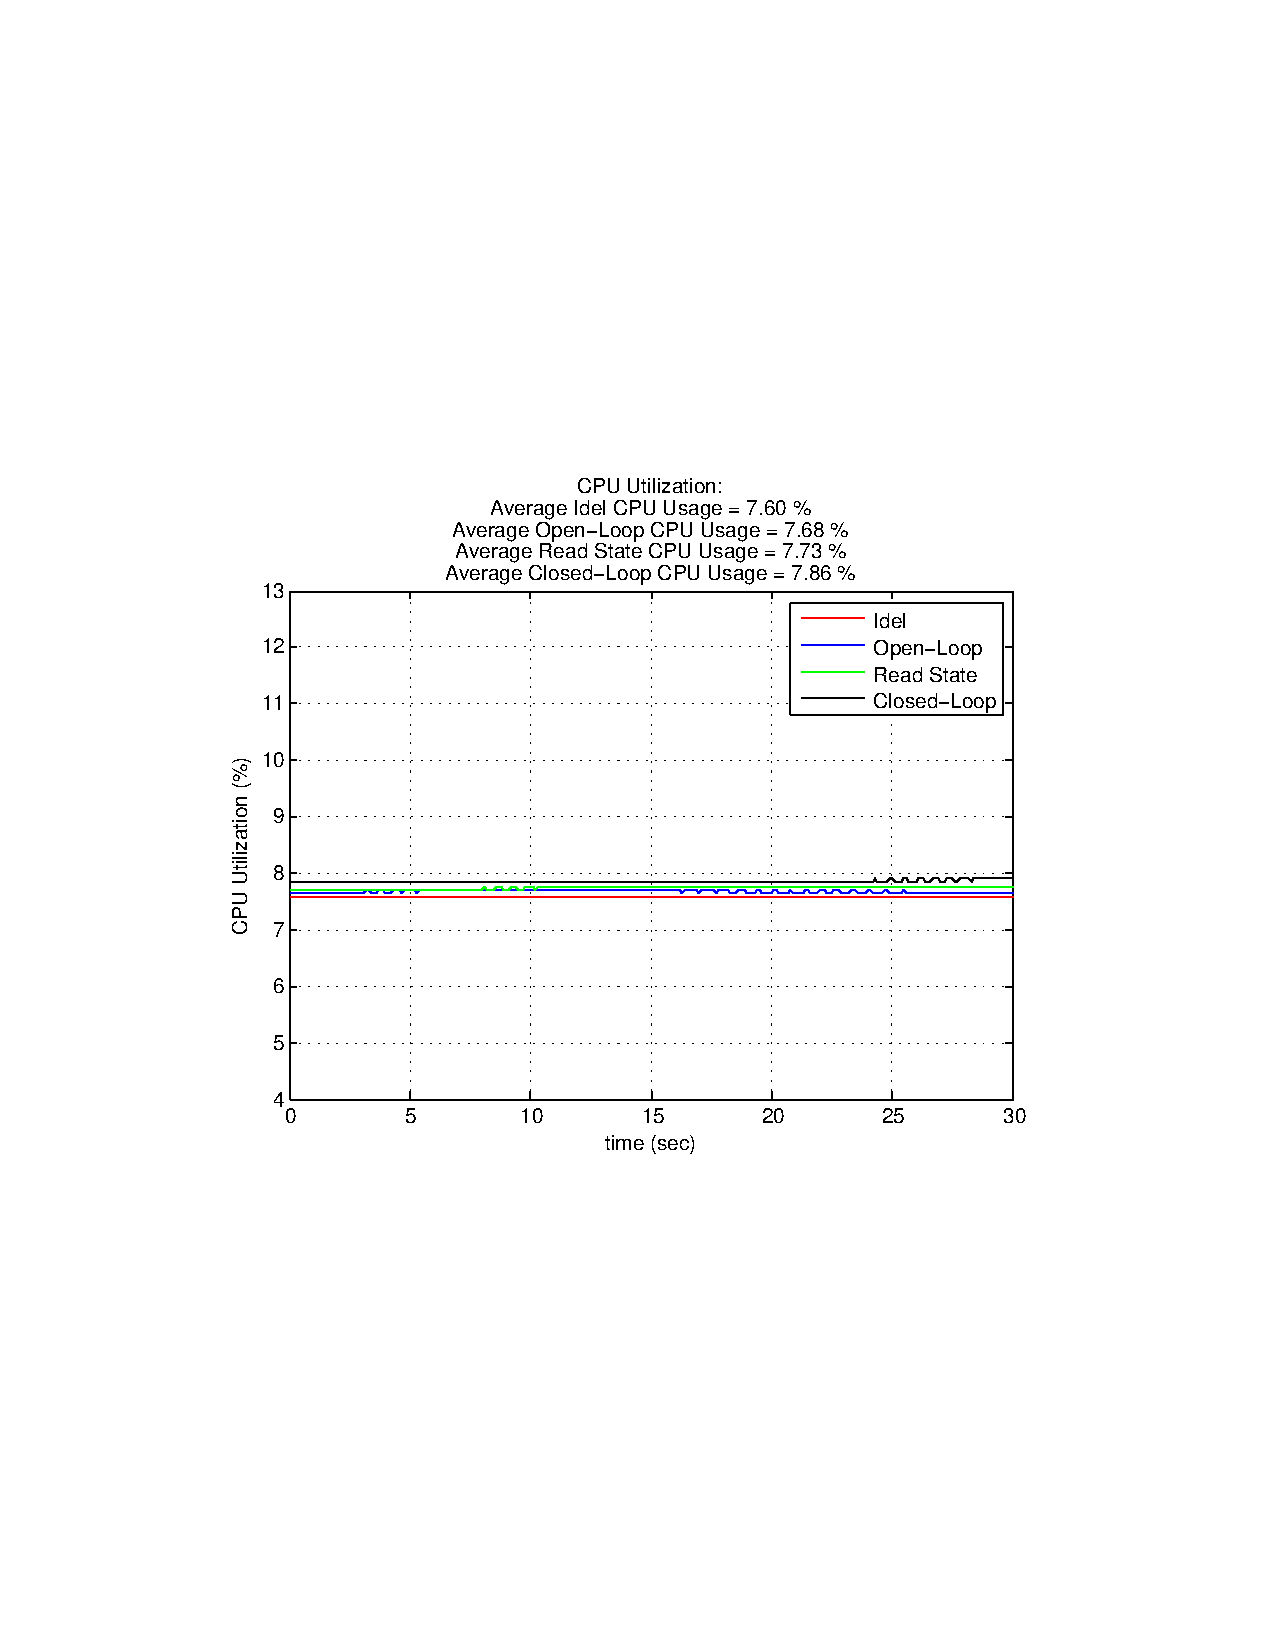
\includegraphics[width=0.6\columnwidth]{./timingData/cpu.pdf}
  \caption{CPU utilization for the Hubo-Ach process when 1) idle, 2) under open-loop control, 3) reading the sensors, and 4) under closed-loop control.  
It is important to note that the cpu utilization stays within 0.3\% when idle and under closed loop control.
This means that the CPU utilization of Hubo-Ach is independent of the external control method.
Thus it will not add more to the CPU load under complex control schemes then under simple ones.}
  \label{fig:timing-getTrigger}
\end{figure}
